% comando para correção ortográfica
%$ aspell -t -c introducao.tex --encoding=utf-8 --lang=pt_BR

\chapter{Introdução}

\section{Problemática}
O consumo de jogos foi crescente nos últimos 5 anos. Como podemos ver na figura
\ref{fig:esa_graph_2017} das pesquisas da ESA,
em 2016 o consumidor norte americano gastou em torno de $30.4$
bilhões de dólares na indústria dos jogos. No mesmo ano, as companhias de jogos
norte americanas adicionaram mais de 11.7 bilhões de dólares na \textit{GDP}
do país \cite{entertainment2017essential}.
\begin{figure}[H]
    \centering
    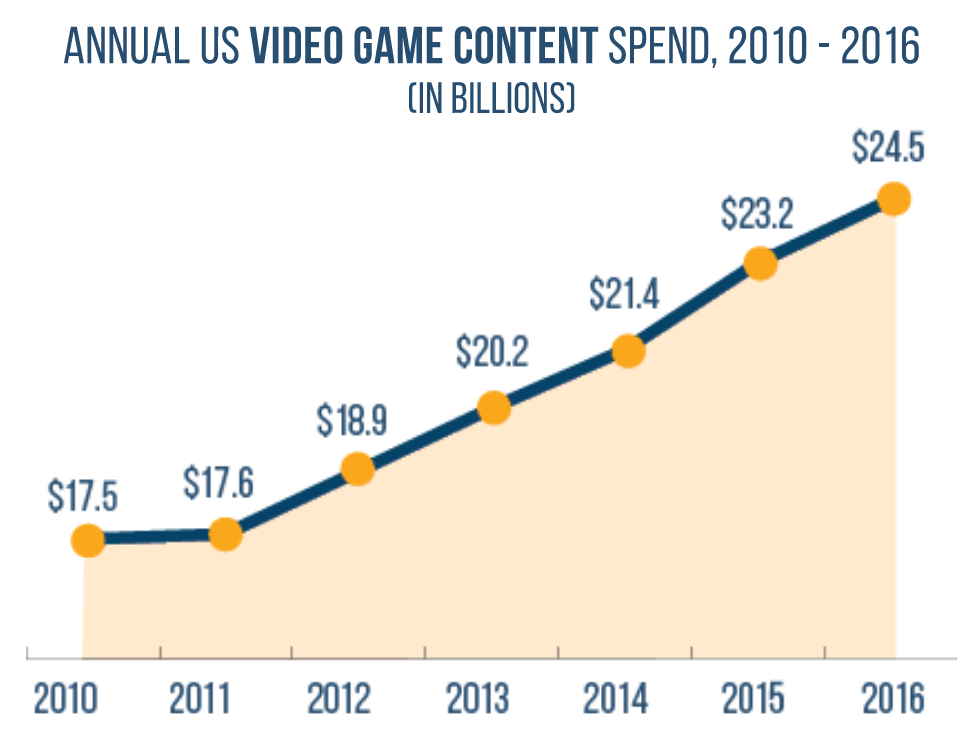
\includegraphics[width=0.5\textwidth]{figuras/ESAGraph2017.png}
    \caption{Consumo com conteúdo de jogos\cite{entertainment2017essential}}
    \label{fig:esa_graph_2017}
\end{figure}

Os investimentos nos jogos também são crescentes neste
período \cite{entertainment2017essential}, um dos jogos com mais investimentos é
o \textit{GTAV} que em desenvolvimento e marketing gastou cerca de $265$
milhões de dólares \cite{villapaz2013gta}. Os jogos tendem a ser cada vez mais
detalhados e complexos, o custo de desenvolvimento também aumenta.
No desenvolvimento de jogos há vários profissionais envolvidos para criar
o conteúdo dos jogos, com equipes de programadores, designers,  roteiristas,
entre outros. A força de trabalho costuma ser a parte mais cara da
criação do jogo.


Quanto mais conteúdo um jogo oferece para o jogador explorar, tecnicamente 
mais tempo o jogador irá usar consumindo o jogo \cite{fernando2009costas}, tendo um engajamento maior.
E jogos com mais tempo de jogatina costumam ser os mais rentáveis, porém,
a maneira tradicional para produzir trabalho artístico demanda tempo. Na maneira
tradicional o jogo é polido e desenhado manualmente por uma equipe de artistas gráficos. Em alguns casos 
quando o jogo exige muito conteúdo, essa prática pode ser inviável.


\section{Apresentação}
O trabalho em questão tem a finalidade de implementar um algoritmo,
que forme proceduralmente relevo para jogos, sem 
interferência do desenvolvedor de jogos neste processo.
O terreno gerado precisa conter aspectos de relevos diferentes, chamados de biomas,
estes biomas devem estar separados em regiões e quando ocorrer uma fronteira
entre biomas distintos, ela deve ser contínua (sem paredões ou mudanças bruscas na altitude),
caso contrário um jogador que manipula uma entidade terrestre teria problemas para 
transitar de um bioma para outro.

Uma maneira de conseguir diminuir os gastos no desenvolvimento de conteúdo, é 
gerando os mesmos proceduralmente, as chamadas técnicas de \textit{PCG}. 
\textit{PCG} é usar algoritmos para gerar o conteúdo \cite{shaker2016procedural}.
Uma aplicação bem comum do \textit{PCG} é a criação de relevos e mapas de altura,
desta maneira não é necessário uma pessoa modelar manualmente a altura do
terreno do cenário.

Com o \textit{PCG} para criar o terreno, é possível criar terrenos com tamanhos
muito maiores que um jogador poderá explorar. Ou seja, não importa o tamanho mas
sim o quão interessante o conteúdo é, mesmo sendo vasto o jogador precisa iniciativas
para explorá-lo.
Hoje temos diversos exemplos de jogos que fazem uso dessa técnica
para criar um cenário pseudo-infinitos, entre eles, \textit{Limit Theory}. Nele
são criados pseudo-infinitos sistemas planetários, de forma procedural, e em cada
sistema planetário os planetas e seus relevos também são gerados proceduralmente
\cite{abreu1990toward}.

O jogo \textit{minecraft} tem uma implementação de geração procedural,
seus mundos são de tamanho pseudo-infinito, 
o algoritmo é não assistido, ou seja, sem a intervenção
do usuário na criação do mundo, nele
são gerados múltiplos biomas, em cada um deles existe uma manipulação diferente
do ruído para recriar as características do bioma. Mesmo em seu mundo
minimalista, o jogador consegue reconhecer o bioma \cite{short2012teaching}.
Na figura \ref{fig:biomesminecraftgameplay}.
Foi usado o sistema online \textit{Chunk Base} para 
ilustrar fronteiras entre biomas, cada cor no mapa é um bioma \ref{fig:chunkbasebiomes}.


\begin{figure}[H]
    \centering
    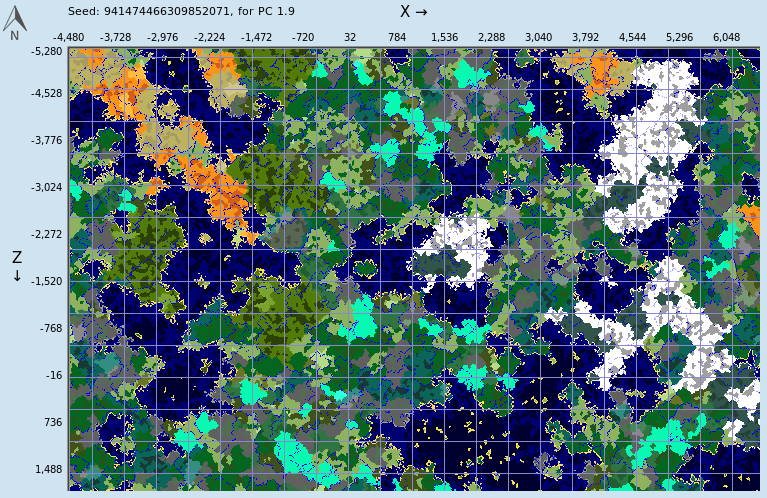
\includegraphics[width=0.7\textwidth]{figuras/chunkbasebiomes.png}
    \caption{Mapa de biomas para mundo virtual do \textit{minecraft}}
    \label{fig:chunkbasebiomes}
\end{figure}

\begin{figure}[H]
    \centering
    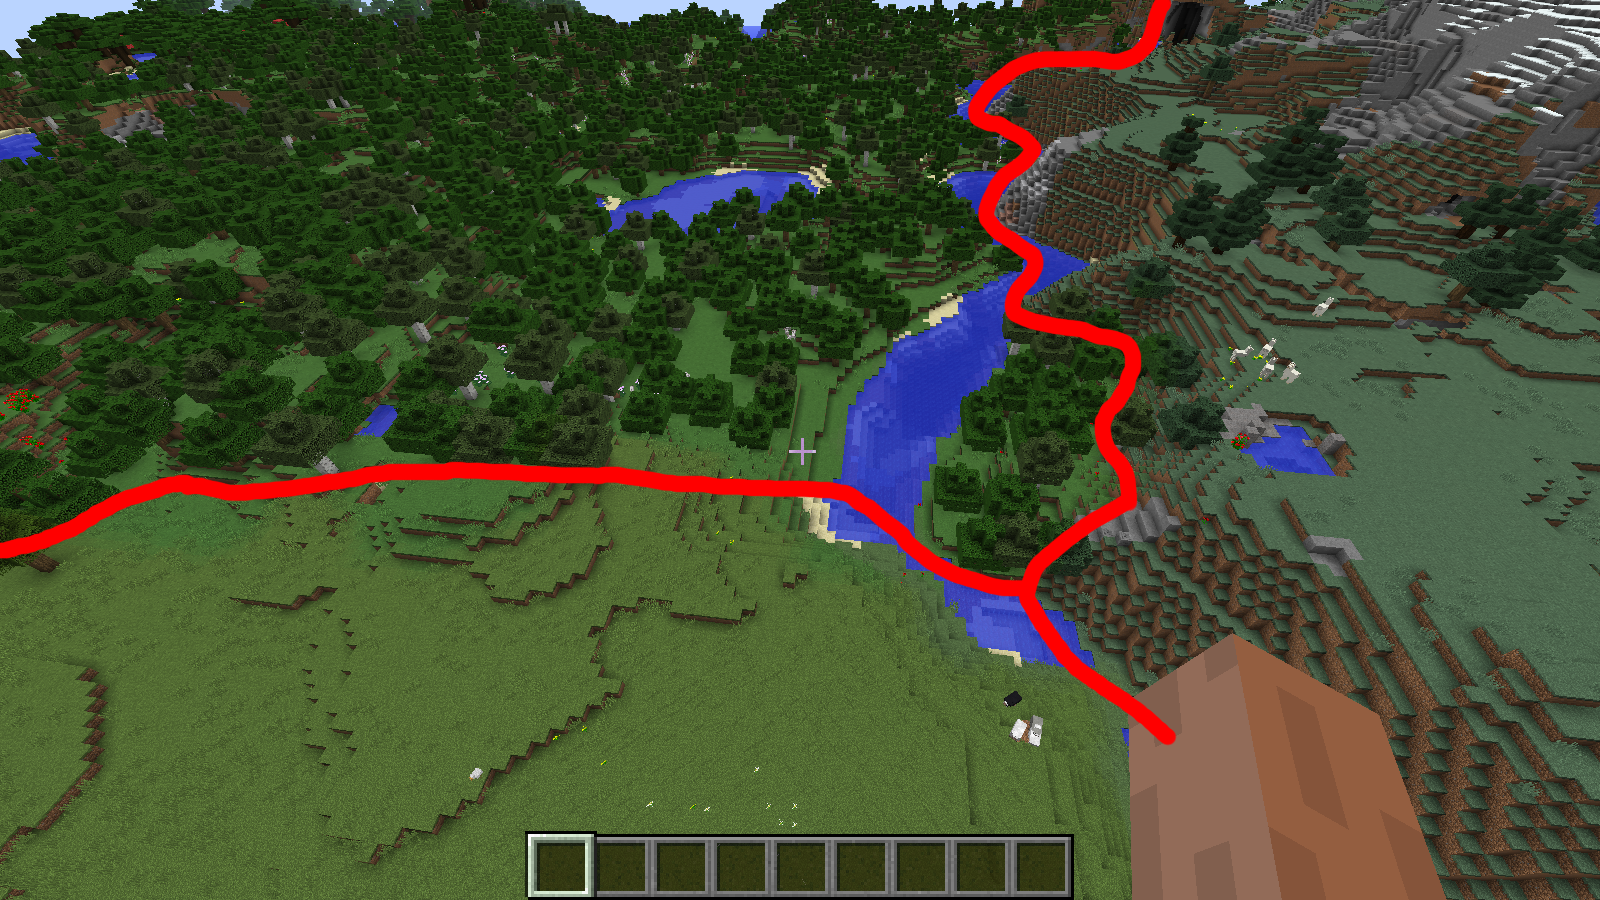
\includegraphics[width=0.7\textwidth]{figuras/biomesminecraftgameplay.png}
    \caption{Perspectiva de um jogador no \textit{minecraft}, com visão para fronteira entre três biomas}
    \label{fig:biomesminecraftgameplay}
\end{figure}
